\section{Extrapolations to higher luminosity}
\label{sec:extrapolations}

Future runs of the LHC expect to deliver significantly higher instantaneous luminosity than current operations. To cope with these harsher data-taking conditions, upgrades to the muon spectrometer are planned. In Long Shutdown 2 (LS2), which is scheduled to start in 2018, the current endcap small wheels will be replaced by the New Small Wheels (NSW) equipped with small Thin Gap Chambers and MicroMegas detectors. In Long Shutdown 3, which is scheduled to start near 2022, the MDT electronics are being considered for replacement, and additional coverage for the barrel muon trigger system is under consideration.

A crucial ingredient in the planning of these upgrades is the hit rate of incident particles the detectors are expected to receive. This note presents an expected rate in the hottest regions of the MS as extrapolated from data-taking in 2015. This extrapolation does not address potential changes in the shielding of the MS, which can have a large effect and must be characterized with simulation. The hottest regions of the MS in 2015 data are the innermost regions of the endcap inner small wheel (CSL1, CSS1) and endcap middle big wheel (EML1, EMS1).

The prediction is performed by considering the hit rates in 2015 data-taking as a function of the instantaneous luminosity, fitting the linear dependence, and extrapolating to higher luminosity. These rates are shown in Figures~\ref{} with linear fits overlaid.

The parameters of the linear fit depend on the number of filled bunches in the LHC, as expected. The maximum number of filled bunches in 2015 is 2232 bunches, whereas Run 3 of the LHC is expected to fill at most 2808 bunches, and the HL-LHC is expected to fill at most 3564 bunches. To extrapolate to more filled bunches, the fitted slopes are considered for 2015 runs with as few as 447 filled bunches and as many as 2232 bunches, and the dependency is extracted by fitting this spectrum to a first-order inverse power law, as shown in Figure~\ref{fig:extrapolations-slope-vs-bunches}. 

\begin{figure}
  \begin{center}
    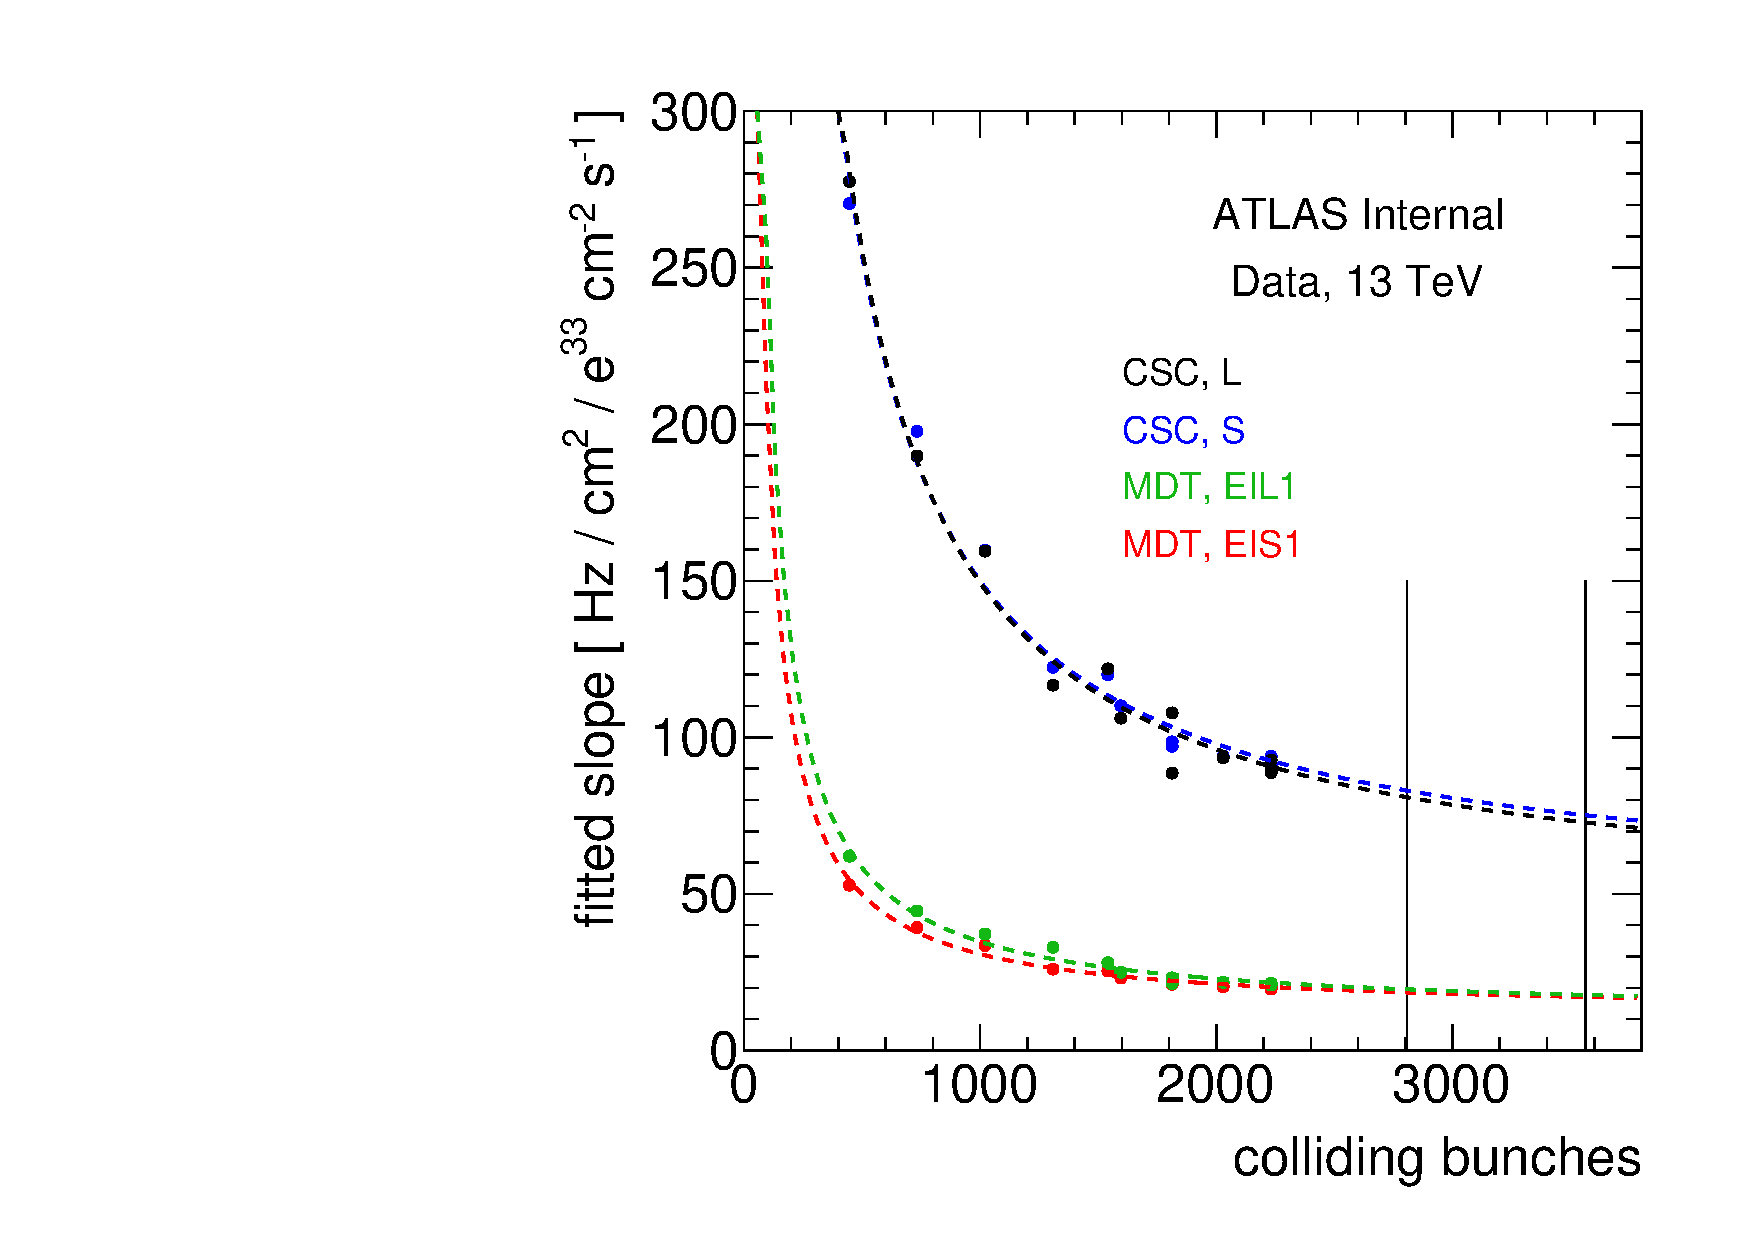
\includegraphics[width=0.45\textwidth]{./figures/slope_vs_bunches.pdf}
    \caption{The fitted slope as a function of the number of colliding bunches for various runs in the hottest MDT and CSC chambers. The spectra are fitted to $A + B/x$, where $x$ is the number of bunches.}
    \label{fig:extrapolations-slope-vs-bunches}
  \end{center}
\end{figure}



